\documentclass[9pt,twoside,lineno]{pnas-new}
% Use the lineno option to display guide line numbers if required.

\templatetype{pnassupportinginfo}
% \readytosubmit %% Uncomment this line before submitting, so that the instruction page is removed.

\title{Your Main Manuscript Title}
\author{Author1, Author2 and Author3 (Complete author list)}
\correspondingauthor{Corresponding Author Name.\\E-mail: author.two@email.com}

\begin{document}

%% Comment/remove this line before generating final copy for submission
%% \instructionspage

\maketitle

%% Adds the main heading for the SI text. Comment out this line if you do not have any supporting information text.
\SItext


\subsection*{Subhead}
Type or paste text here. This should be additional explanatory text such as an extended technical description of results, full details of mathematical models, extended lists of acknowledgments, etc.

\section*{Heading}
\subsection*{Subhead}
Type or paste text here. You may break this section up into subheads as needed (e.g., one section on ``Materials'' and one on ``Methods'').

\subsection*{Materials}
Add a Materials subsection if you need to.

\subsection*{Methods}
Add a Methods subsection if you need to.


%%% Each figure should be on its own page
% \begin{figure}
% \centering
% \includegraphics[width=\textwidth]{example-image}
% \caption{First figure}
% \end{figure}

% \begin{figure}
% \centering
% 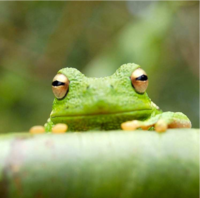
\includegraphics[width=\textwidth]{frog}
% \caption{Second figure}
% \end{figure}

\begin{table}\centering
\caption{This is a table}

\begin{tabular}{lrrr}
Species & CBS & CV & G3 \\
\midrule
1. Acetaldehyde & 0.0 & 0.0 & 0.0 \\
2. Vinyl alcohol & 9.1 & 9.6 & 13.5 \\
3. Hydroxyethylidene & 50.8 & 51.2 & 54.0\\
\bottomrule
\end{tabular}
\end{table}

%%% Add this line AFTER all your figures and tables
\FloatBarrier

\movie{Type caption for the movie here.}

\movie{Type caption for the other movie here. Adding longer text to show what happens, to decide on alignment and/or indentations.}

\movie{A third movie, just for kicks.}

\dataset{dataset_one.txt}{Type or paste caption here.}

\dataset{dataset_two.txt}{Type or paste caption here. Adding longer text to show what happens, to decide on alignment and/or indentations for multi-line or paragraph captions.}

\bibliography{pnas-sample}

\end{document}